
\section{Settings (To Be Updated)}
% Having implemented the algorithm, we now describe the experiment configuration and results in this chapter.
The two main measurements for the performance of our new architecture are learning efficiency and transfer learning capability.
We conducted several different experiments to highlight each aspect of the algorithm.

We use GVG-AI Framework for our experiments, which was created for the General Video Gamea AI Competition\footnote{http://www.gvgai.net/}, 
a game environment for an agent that should be able to play a wide variety of games without knowing which games are to be played.
The underlying language is the Video Game Definition Language (VGDL), which is a high-level description language for 2D video games providing a platform for computational intelligence research (\cite{Schaul2013}).
The VGDL allows users to easily craft their own environments, which makes us possible to do various experiments without relying on the default environments.
The base game is a maze implemented using VGDL game platform. 

As shown in Figure \ref{VGDL_sample}, there are 3 different types of cells: 
a goal cell, walls and paths. The agent can take 4 different actions: up, down, right and left.  
The environment is not known to the agent in advance, and it attempts to find the goal by exploring the environment.
The agent receives -1 in any states except the goal state, where it gains a reward of 10. 

\begin{figure}[!ht!b]
\centering
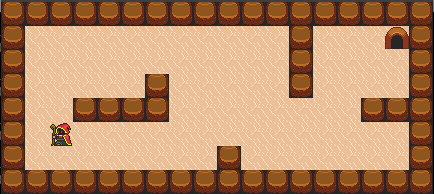
\includegraphics[width=0.5\textwidth]{./figures/experiment1}
\caption{VGDL game example}
\label{VGDL_sample}
\end{figure}
  
% No dynamic enemies,
% \textcolor{red}{TODO OPENAI paper citation}
% The game is formalised as MDP as follows:
% I conducted a number of experiments to highlight a different aspects of the algorithms. 
% To compare the performance of our algorithm, I ran Q-learning, the most commonly used RL algorithm, in the same senarios as a bench mark. 

\section{Benchmark (To Be Updated)}

We compare the performance of our algorithm with existing reinforcement learning techniques. 
Q-learning is most widely used technique for reinforcement learning. However comparision with q-learning might not be fair 
since our algorithm has one extra assumptions: the agent knows surrounding information (whether there are walls in adjacent cells), 
which is not a common assumption for RL.
Another benchmark is tile coding, which is a type of linear function approximation techniques described in Chapter XX. 

\section{Experiment Results (To Be Updated)}
\label{learning_evaluation}

\subsection{Experiment1}

\begin{figure}[!htb]
\centering
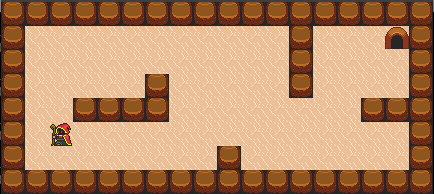
\includegraphics[width=0.5\textwidth]{./figures/experiment1}
\caption{Enviroment for experiment 1}
\label{experiment1}
\end{figure}
    

\begin{figure}[!htb]
\centering
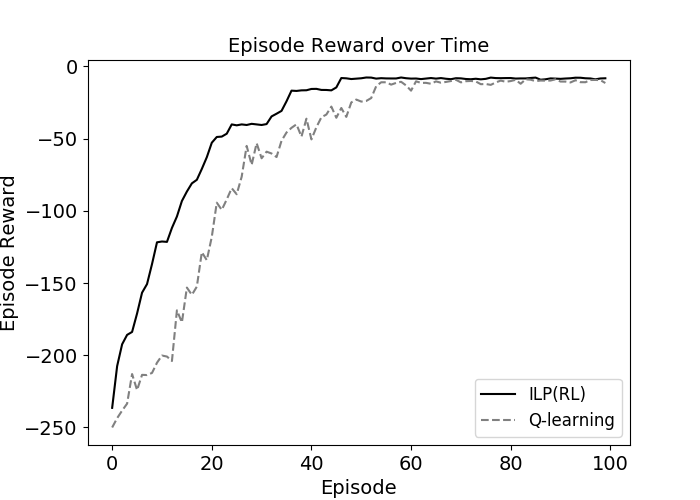
\includegraphics[width=1.0\textwidth]{./figures/experiment1_training}
\caption{Comparison of training performance between my algorithm and Q-learning}
\label{experiment1_training}
\end{figure}


\begin{figure}[!htb]
\centering
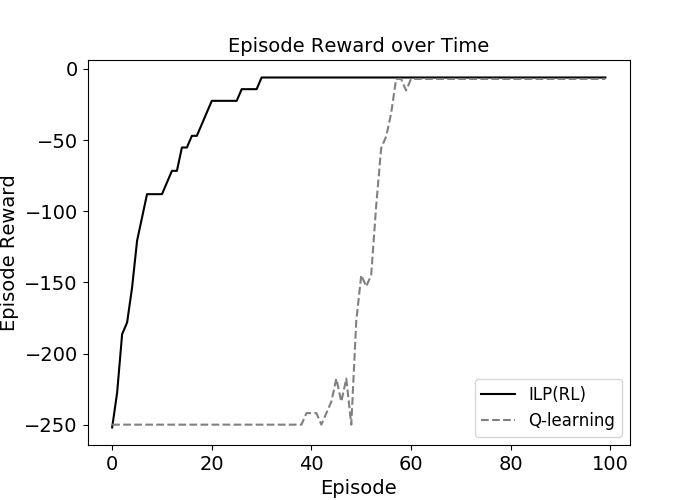
\includegraphics[width=1.0\textwidth]{./figures/experiment1_test}
\caption{Comparison of test performance between my algorithm and Q-learning}
\label{experiment1_test}
\end{figure}
    

Experiment 1 update H

First H

TODO Insert Hypothesis here

Last H after XX iterations. 

TODO Insert Hypothesis here

% \subsection{Evaluation Methods}

Converge to optimal policy faster than Q-learning.


\subsection{Experiment2}

TODO Comparison with Tile Coding
% The first experiment might not be a fair comparision between our algorithm and Q-learning, since our algorithm has extra information about the surrounding information.
% In order to have the same assumptions, we use function approximation for Q-learning. 
% Linear function approximation. 
% \begin{figure}[!htb]
% \centering
% 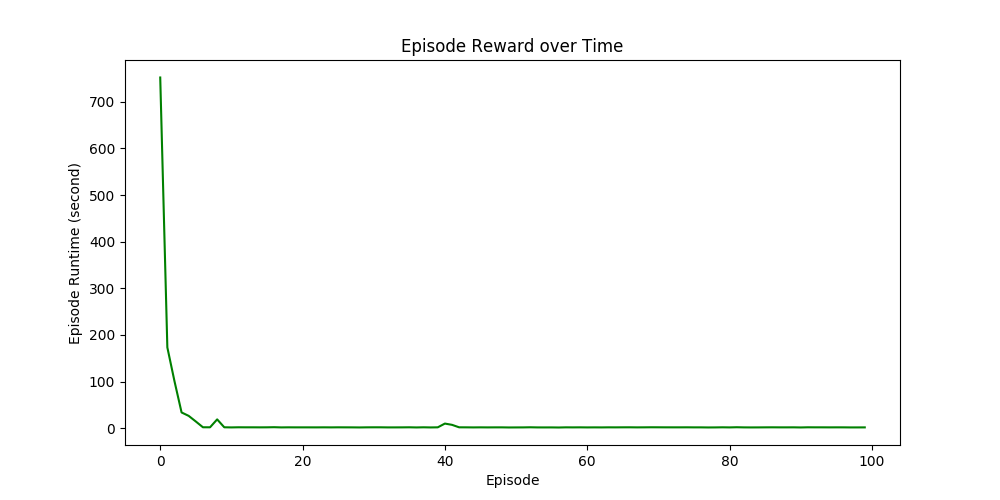
\includegraphics[width=1.0\textwidth]{./figures/placeholder}
% % 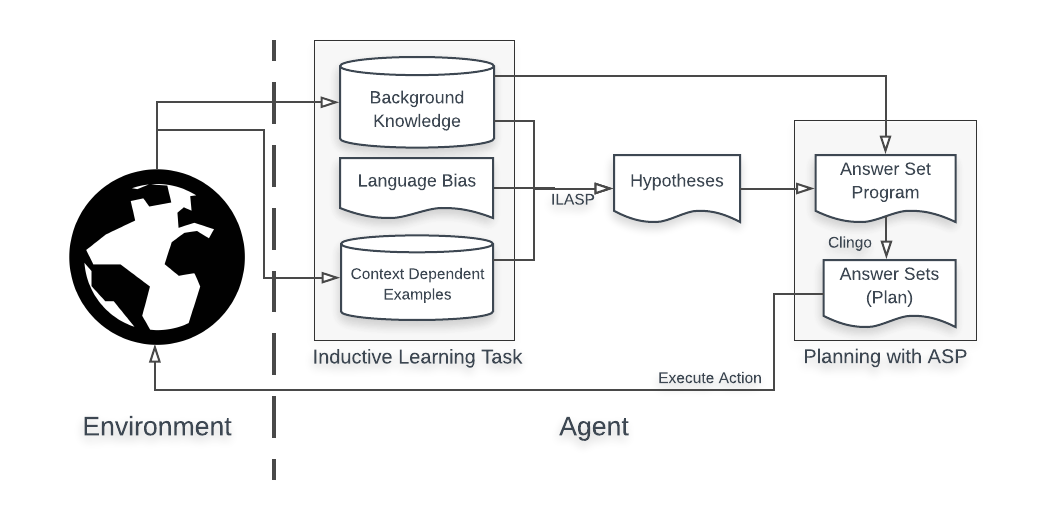
\includegraphics[width=10cm, height=9cm]{./figures/architecture}
% \caption{PLACEHOLDER}
% \label{proposed_architecture}
% \end{figure}
\newpage

\subsection{Experiment3}
Experiment 3 Optimal path learning
This experiment is conducted to see if the agent does not get stuck on a suboptimal path. 

The game is designed such that 

Teleport. 

\begin{figure}[!htb]
\centering
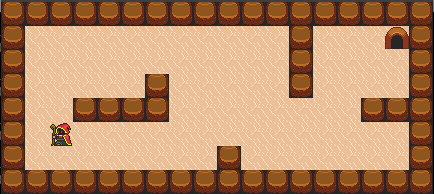
\includegraphics[width=0.5\textwidth]{./figures/experiment1}
\caption{Enviroment for experiment 1}
\label{experiment1}
\end{figure}
    

\begin{figure}[!htb]
\centering
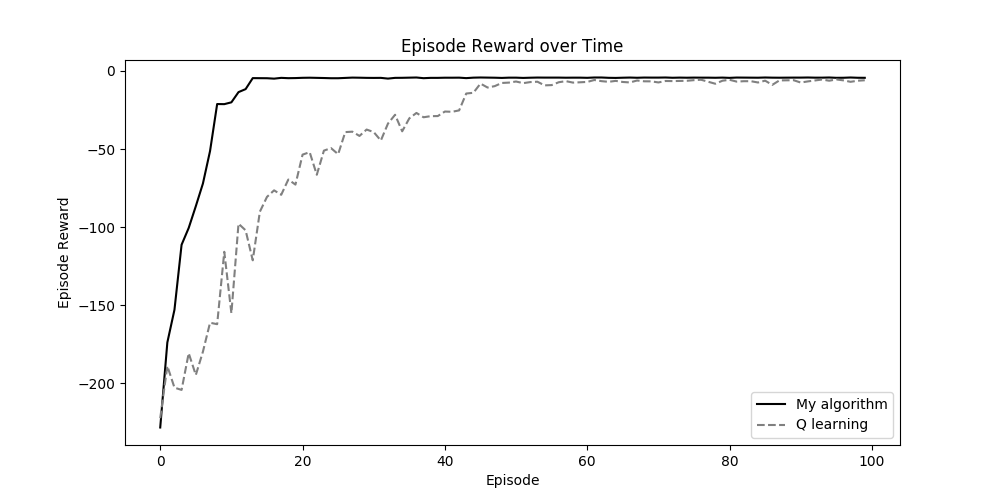
\includegraphics[width=1.0\textwidth]{./figures/experiment3_training}
\caption{Comparison of training performance between my algorithm and Q-learning}
\label{experiment1_training}
\end{figure}

\begin{figure}[!htb]
\centering
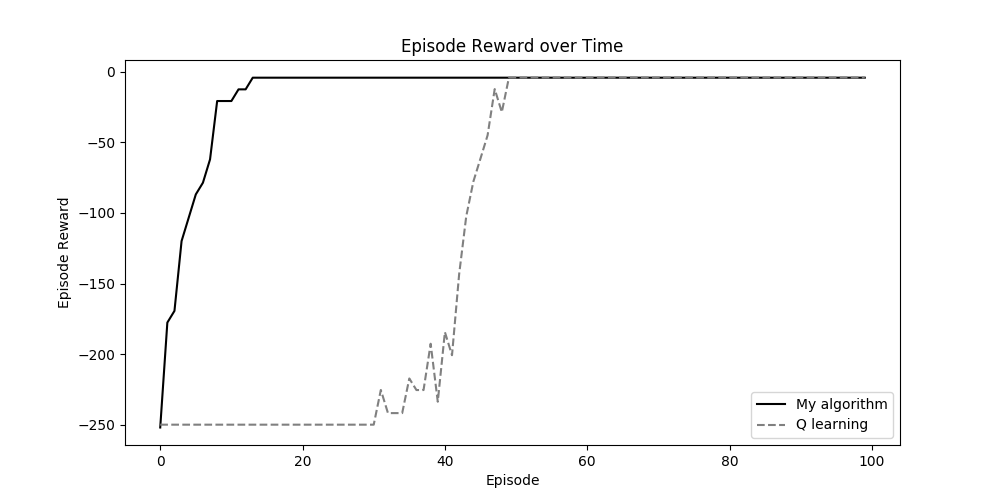
\includegraphics[width=1.0\textwidth]{./figures/experiment3_test}
\caption{Comparison of test performance between my algorithm and Q-learning}
\label{experiment1_test}
\end{figure}
        
    
\newpage
\section{Transfer Learning Evaluation}
\label{transfer_learning}

\subsection{Experiment4}

\begin{figure}[!htb]
\centerline{
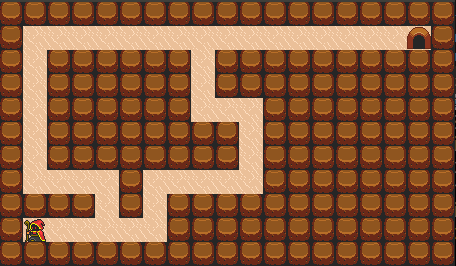
\includegraphics[width=0.5\textwidth]{./figures/experiment4_before}
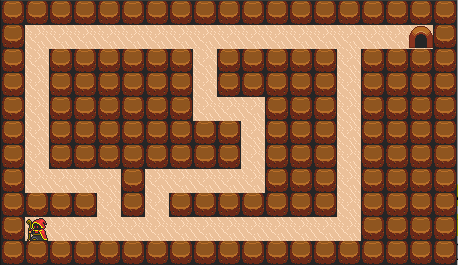
\includegraphics[width=0.5\textwidth]{./figures/experiment4_after}
}
\caption{Before (left) and after (right) transfer learning}
\label{experiment4}
\end{figure}    

Finally, we investigated the potentials of transfer learning betweeen similar environments. 

The goal position is the same as in the first game, but the routes to the goal is different. 

Experiment 4 Transfer learning 
    1 update B
    2 update H

% \textsf{\#modeb(1, link(var(cell), var(cell)), (positive)).}

\begin{figure}[!htb]
\centering
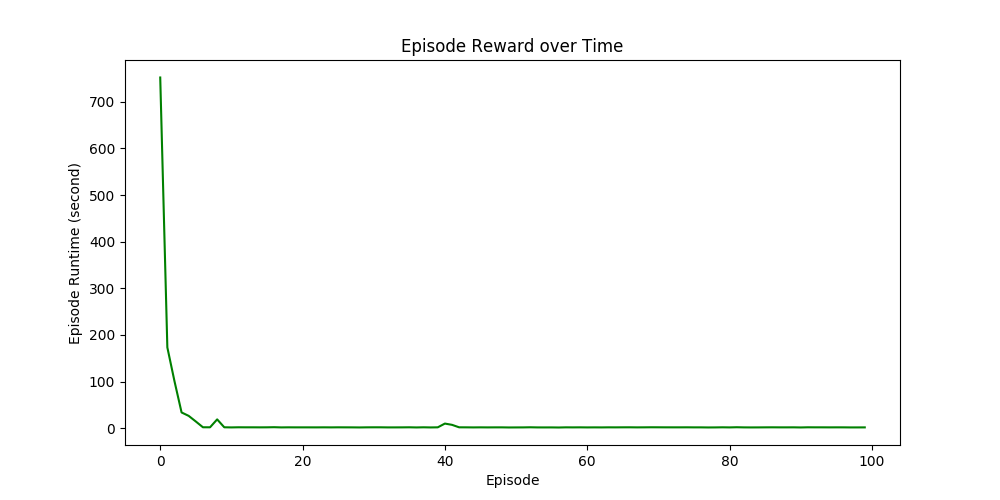
\includegraphics[width=1.0\textwidth]{./figures/placeholder}
% 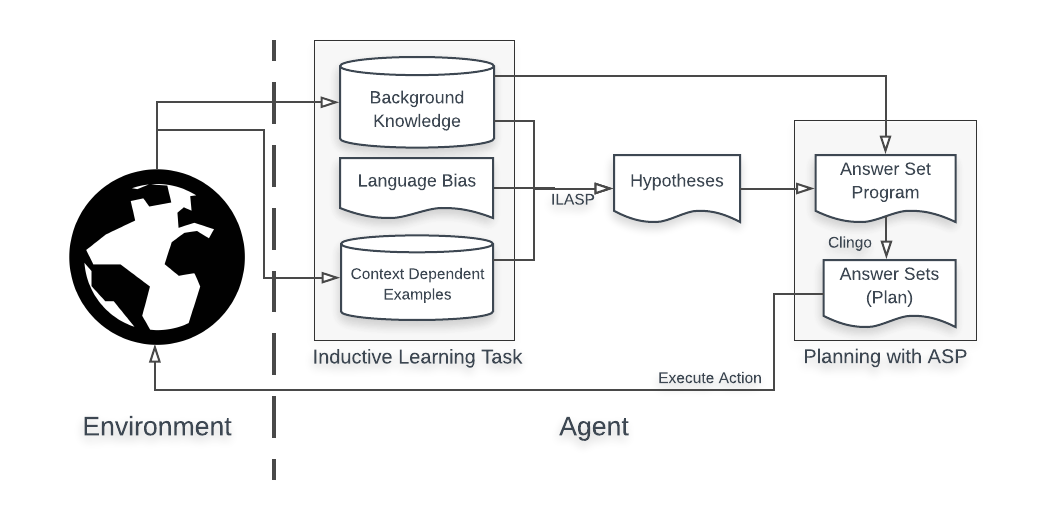
\includegraphics[width=10cm, height=9cm]{./figures/architecture}
\caption{PLACEHOLDER}
\label{proposed_architecture}
\end{figure}


% \subsection{Results}

% \subsection{Discussion}
% \subsubsection{Strengths}

% \subsection{Limitations}

% You have to define the search space for H

% Learning ILASP is known to be less scalable. 

% ILASP learning is quite slow

% Another limitation is training time. Unlike existing reinforcement learning, 
% out algorithm refines hypothesis at every time steps within the same episode. 
% Thus even though the efficiency in terms of the number of iteration is higher, 
% training time within each iteration tends to be lower. 
% As stated in XXX